 \section{Eredmények} 
	\subsection{MATLAB implementációk}
	A referenciaként szolgáló MATLAB algoritmus lineáris programszervezést
	alkalmazva az elérhető fajlagos futási idő $\sim100 ms$.
	
	A kód minimális változtatásával elérhető a párhuzamos végrehajtás. Ezt a
	\texttt{for} ciklusok Parallel Toolbox beli \texttt{parfor} utasítására
	cserélve érhetjük el. 4 processzormaggal rendelkező PC esetén ilyenkor
	közel a negyedére csökken a futási idő.
	
	\subsection{OpenCL implementációk}
	OpenCL keretrendszer segítségével írt programot a GPU-n futtatva a
	\ref{table:openresult} táblázatban látható eredményeket kapjuk.
	Csupán a globális memóriát használva a referenciához képest romlik a
	teljesítmény. Ezt a videókártya prediktív cache nélküli kialakításának és a
	globális memórája okozta kiéheztetésnek tudhatjuk be.
	A lokális memória használata a futási időt drasztikusan le tudja
	csökkenteni, ami a korábban ismertetett memória szervezési gondolatok
	helyességét igazolja.
	 
	\begin{table*}[!b]
	\renewcommand{\arraystretch}{1.2}
	% if using array.sty, it might be a good idea to tweak the value of
	% \extrarowheight as needed to properly center the text within the cells
	\caption{OpenCL futási idő eredmények $12\times12$ mérési pontra}
	\label{table:openresult}
	% Some packages, such as MDW tools, offer better commands for making tables
	% than the plain LaTeX2e tabular which is used here.
	\centering
	\begin{tabular}{l|r|r|r}
	 & Globális memória & Lokális memória, ha befér & Lokális memória bufferelés\\ \hline
	\parbox{2.5cm}{Globális tranzakciók száma átlagosan} & $12 \times 12\times 32.3$
	& $12 \times 12 \times 32.3$ & $12 \times 12 \times 32.3$\\
	\parbox{2.5cm}{Lokális tranzakciók száma átlagosan} & 0 &
	$0.48 \times 12 \times 12 \times 30$ & $2.08 \times 12 \times12 \times 32.3$\\
	Futási idő & 5990 ms & 2530 ms & 510 ms\\
	Fajlagos futási idő & 410 ms & 170 ms & 3.5 ms 
	\end{tabular}
	\end{table*}
	
	\begin{figure*}[!t]
		\centering
		\subfloat[Mérési eredmény]{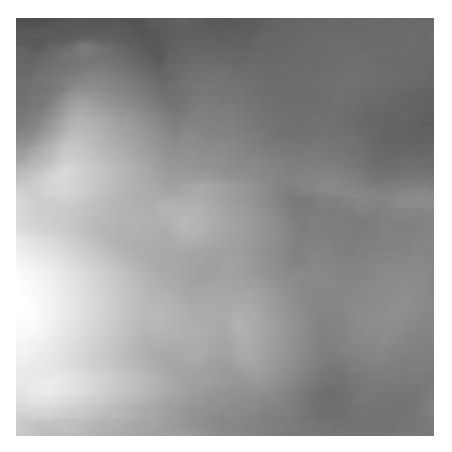
\includegraphics[width=0.45\columnwidth]{kepek/afm200.eps}%
		\label{fig_first_case}}
		\hfil
		\subfloat[Szimulációs eredmény]{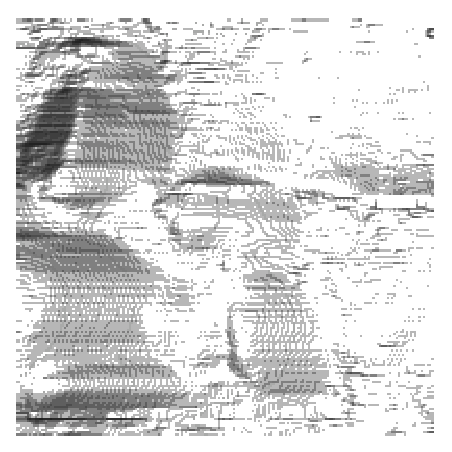
\includegraphics[width=0.45\columnwidth]{kepek/efm200.eps}%
		\label{fig_second_case}}
		\caption{Méréssel kapott felület (balra) és szimulációval kapott töltéstérkép}
		\label{fig_sim}
	\end{figure*}
	
